\documentclass{standalone}
\usepackage[utf8]{inputenc}
\usepackage{pgfplots}
\DeclareUnicodeCharacter{2212}{−}
\usepgfplotslibrary{groupplots}
\usepgfplotslibrary{dateplot}
\usetikzlibrary{patterns}
\usetikzlibrary{shapes.arrows}
\pgfplotsset{compat=newest}
\begin{document}
% This file was created by tikzplotlib v0.9.1.
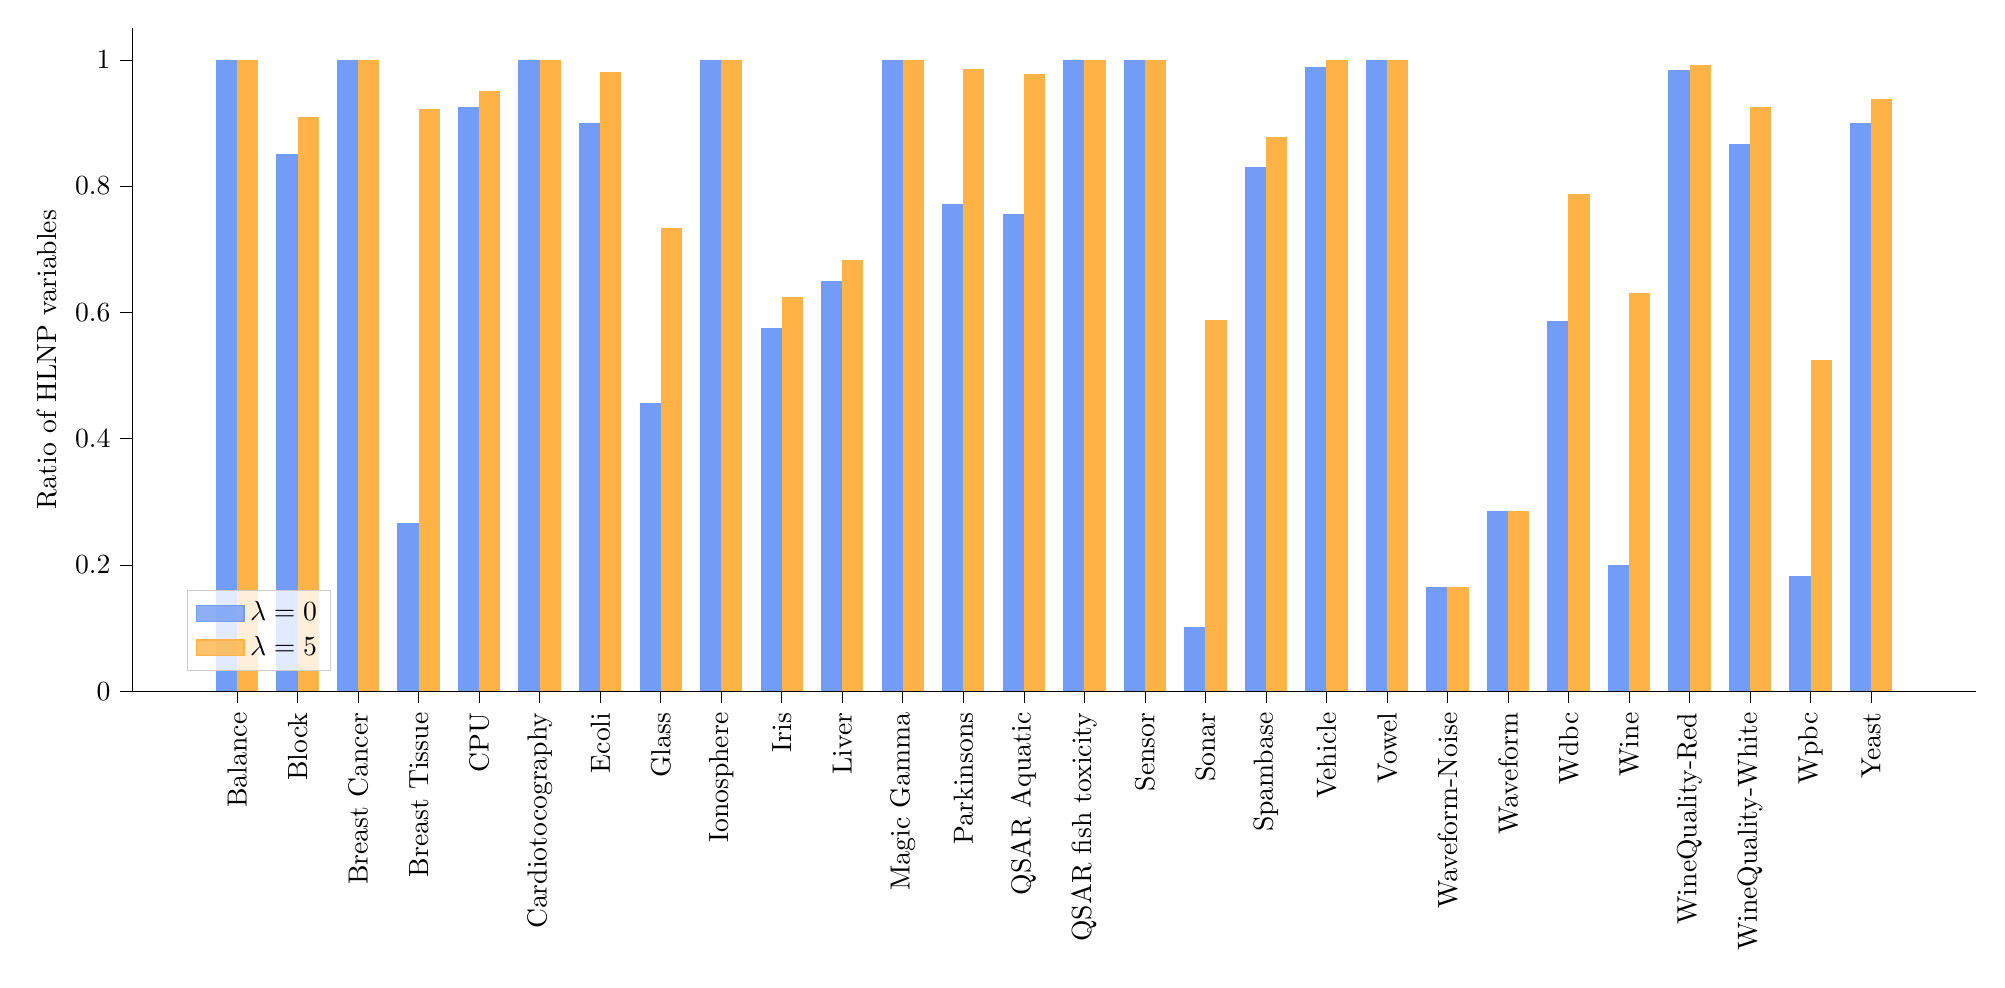
\begin{tikzpicture}

\definecolor{color0}{rgb}{0.447058823529412,0.611764705882353,0.96078431372549}
\definecolor{color1}{rgb}{1,0.701960784313725,0.274509803921569}

\begin{axis}[
height=10cm,
legend cell align={left},
legend style={fill opacity=0.8, draw opacity=1, text opacity=1, draw=white!80!black},
tick align=outside,
tick pos=left,
width=25cm,
x grid style={white!69.0196078431373!black},
xmin=-1.385, xmax=29.085,
xtick style={color=black},
xtick={0.35,1.35,2.35,3.35,4.35,5.35,6.35,7.35,8.35,9.35,10.35,11.35,12.35,13.35,14.35,15.35,16.35,17.35,18.35,19.35,20.35,21.35,22.35,23.35,24.35,25.35,26.35,27.35},
xticklabel style = {rotate=90.0},
xticklabels={Balance,Block,Breast Cancer,Breast Tissue,CPU,Cardiotocography,Ecoli,Glass,Ionosphere,Iris,Liver,Magic Gamma,Parkinsons,QSAR Aquatic,QSAR fish toxicity,Sensor,Sonar,Spambase,Vehicle,Vowel,Waveform-Noise,Waveform,Wdbc,Wine,WineQuality-Red,WineQuality-White,Wpbc,Yeast},
y grid style={white!69.0196078431373!black},
ylabel={Ratio of HLNP variables},
ymin=0, ymax=1.05,
ytick style={color=black},
legend pos = south west,
axis x line*=bottom,
axis y line*=left,
]
\draw[draw=none,fill=color0] (axis cs:0,0) rectangle (axis cs:0.35,1);
\draw[draw=none,fill=color0] (axis cs:1,0) rectangle (axis cs:1.35,0.85);
\draw[draw=none,fill=color0] (axis cs:2,0) rectangle (axis cs:2.35,1);
\draw[draw=none,fill=color0] (axis cs:3,0) rectangle (axis cs:3.35,0.266666666666667);
\draw[draw=none,fill=color0] (axis cs:4,0) rectangle (axis cs:4.35,0.925);
\draw[draw=none,fill=color0] (axis cs:5,0) rectangle (axis cs:5.35,1);
\draw[draw=none,fill=color0] (axis cs:6,0) rectangle (axis cs:6.35,0.9);
\draw[draw=none,fill=color0] (axis cs:7,0) rectangle (axis cs:7.35,0.455555555555555);
\draw[draw=none,fill=color0] (axis cs:8,0) rectangle (axis cs:8.35,1);
\draw[draw=none,fill=color0] (axis cs:9,0) rectangle (axis cs:9.35,0.575);
\draw[draw=none,fill=color0] (axis cs:10,0) rectangle (axis cs:10.35,0.65);
\draw[draw=none,fill=color0] (axis cs:11,0) rectangle (axis cs:11.35,1);
\draw[draw=none,fill=color0] (axis cs:12,0) rectangle (axis cs:12.35,0.771428571428571);
\draw[draw=none,fill=color0] (axis cs:13,0) rectangle (axis cs:13.35,0.755555555555556);
\draw[draw=none,fill=color0] (axis cs:14,0) rectangle (axis cs:14.35,1);
\draw[draw=none,fill=color0] (axis cs:15,0) rectangle (axis cs:15.35,1);
\draw[draw=none,fill=color0] (axis cs:16,0) rectangle (axis cs:16.35,0.101666666666667);
\draw[draw=none,fill=color0] (axis cs:17,0) rectangle (axis cs:17.35,0.829824561403509);
\draw[draw=none,fill=color0] (axis cs:18,0) rectangle (axis cs:18.35,0.988888888888889);
\draw[draw=none,fill=color0] (axis cs:19,0) rectangle (axis cs:19.35,1);
\draw[draw=none,fill=color0] (axis cs:20,0) rectangle (axis cs:20.35,0.165);
\draw[draw=none,fill=color0] (axis cs:21,0) rectangle (axis cs:21.35,0.285714285714286);
\draw[draw=none,fill=color0] (axis cs:22,0) rectangle (axis cs:22.35,0.586666666666667);
\draw[draw=none,fill=color0] (axis cs:23,0) rectangle (axis cs:23.35,0.2);
\draw[draw=none,fill=color0] (axis cs:24,0) rectangle (axis cs:24.35,0.983333333333333);
\draw[draw=none,fill=color0] (axis cs:25,0) rectangle (axis cs:25.35,0.866666666666667);
\draw[draw=none,fill=color0] (axis cs:26,0) rectangle (axis cs:26.35,0.181818181818182);
\draw[draw=none,fill=color0] (axis cs:27,0) rectangle (axis cs:27.35,0.9);
\draw[draw=none,fill=color1] (axis cs:0.35,0) rectangle (axis cs:0.7,1);
\draw[draw=none,fill=color1] (axis cs:1.35,0) rectangle (axis cs:1.7,0.91);
\draw[draw=none,fill=color1] (axis cs:2.35,0) rectangle (axis cs:2.7,1);
\draw[draw=none,fill=color1] (axis cs:3.35,0) rectangle (axis cs:3.7,0.922222222222222);
\draw[draw=none,fill=color1] (axis cs:4.35,0) rectangle (axis cs:4.7,0.95);
\draw[draw=none,fill=color1] (axis cs:5.35,0) rectangle (axis cs:5.7,1);
\draw[draw=none,fill=color1] (axis cs:6.35,0) rectangle (axis cs:6.7,0.98);
\draw[draw=none,fill=color1] (axis cs:7.35,0) rectangle (axis cs:7.7,0.733333333333333);
\draw[draw=none,fill=color1] (axis cs:8.35,0) rectangle (axis cs:8.7,1);
\draw[draw=none,fill=color1] (axis cs:9.35,0) rectangle (axis cs:9.7,0.625);
\draw[draw=none,fill=color1] (axis cs:10.35,0) rectangle (axis cs:10.7,0.683333333333333);
\draw[draw=none,fill=color1] (axis cs:11.35,0) rectangle (axis cs:11.7,1);
\draw[draw=none,fill=color1] (axis cs:12.35,0) rectangle (axis cs:12.7,0.985714285714286);
\draw[draw=none,fill=color1] (axis cs:13.35,0) rectangle (axis cs:13.7,0.977777777777778);
\draw[draw=none,fill=color1] (axis cs:14.35,0) rectangle (axis cs:14.7,1);
\draw[draw=none,fill=color1] (axis cs:15.35,0) rectangle (axis cs:15.7,1);
\draw[draw=none,fill=color1] (axis cs:16.35,0) rectangle (axis cs:16.7,0.588333333333333);
\draw[draw=none,fill=color1] (axis cs:17.35,0) rectangle (axis cs:17.7,0.87719298245614);
\draw[draw=none,fill=color1] (axis cs:18.35,0) rectangle (axis cs:18.7,1);
\draw[draw=none,fill=color1] (axis cs:19.35,0) rectangle (axis cs:19.7,1);
\draw[draw=none,fill=color1] (axis cs:20.35,0) rectangle (axis cs:20.7,0.165);
\draw[draw=none,fill=color1] (axis cs:21.35,0) rectangle (axis cs:21.7,0.285714285714286);
\draw[draw=none,fill=color1] (axis cs:22.35,0) rectangle (axis cs:22.7,0.786666666666667);
\draw[draw=none,fill=color1] (axis cs:23.35,0) rectangle (axis cs:23.7,0.630769230769231);
\draw[draw=none,fill=color1] (axis cs:24.35,0) rectangle (axis cs:24.7,0.991666666666667);
\draw[draw=none,fill=color1] (axis cs:25.35,0) rectangle (axis cs:25.7,0.925);
\draw[draw=none,fill=color1] (axis cs:26.35,0) rectangle (axis cs:26.7,0.524242424242424);
\draw[draw=none,fill=color1] (axis cs:27.35,0) rectangle (axis cs:27.7,0.9375);

\addlegendimage{area legend,fill=color0, color=color0}
\addlegendimage{area legend,fill=color1, color=color1}
\legend{$\lambda = 0$, $\lambda = 5$}
\end{axis}

\end{tikzpicture}

\end{document}
